\section{Training and Evaluation Details}
\label{app:details}

\subsection{Supervised fine-tuning}
\label{app:sft}

\paragraph{Two SFT runs.}
Supervised fine-tuning consists of two separate 5-epoch runs from the base model. They share the hyperparameters in Table~\ref{tab:app-hparams} and differ in training data (Table~\ref{tab:app-sft-data}). The GUI-only run uses emulator trajectories together with GUI simulator trajectories, and does not use app-native tools. The hybrid run uses the full emulator and simulator mixture, including 1,774 simulator trajectories that interleave app-native tool calls. GUI trajectories use the GUI-only system prompt, whereas hybrid trajectories use a tool-aware system prompt. RL is initialized from the hybrid-run checkpoint.

\paragraph{Training samples.}
Each trajectory yields one training sample per step. A sample contains the task instruction, the interaction history up to that step, and a target turn consisting of a \texttt{Thought:} paragraph followed by one tool call. The three most recent screenshots are retained as images; older screenshots are replaced with the text ``This screenshot has been collapsed.'' The full mixture contains 118,582 step-level samples. SFT screenshots are fed at their native $1080\times2400$ resolution, and the model predicts coordinates in a normalized $999\times999$ space.

\paragraph{Action space.}
The GUI-only run uses the \texttt{mobile\_use} tool with actions \texttt{click}, \texttt{long\_press}, \texttt{swipe}, \texttt{type}, \texttt{answer}, \texttt{system\_button} (Back, Home, Menu, or Enter), \texttt{wait}, and \texttt{terminate} (success or failure). The hybrid run adds app-native tools, including actions such as \texttt{clock\_\_create\_alarm} and \texttt{notes\_\_create\_note}. An application's tool catalog is available only while that application is in the foreground, so the policy chooses between a GUI action and an available app-native action at each step.



\begin{table}[H]
\centering
\small
\caption{Training hyperparameters. SFT values are shared by both runs; -- indicates that a setting does not apply.}
\label{tab:app-hparams}
\setlength{\tabcolsep}{3pt}
\begin{tabular}{p{0.27\linewidth}p{0.32\linewidth}p{0.32\linewidth}}
\toprule
Hyperparameter & SFT & RL \\
\midrule
Framework & Megatron-SWIFT & verl \\
Objective & Next-token prediction & DAPO (group-relative) \\
Trainable parameters & LLM (vision frozen) & LoRA \\
Optimizer & Adam ($\beta_1{=}0.9$, $\beta_2{=}0.95$) & AdamW \\
Weight decay / gradient clip & 0.1 / 1.0 & 0.1 / 1.0 \\
Learning rate & $5\times10^{-6}$ & $1\times10^{-6}$ \\
Schedule & Cosine; 3\% warmup; minimum $10^{-7}$ & 40 warmup steps \\
Batch size & 32 (microbatch 1) & 64 tasks $\times$ 8 rollouts \\
Training length & 5 epochs & 150 steps (budget 300); 2 updates each \\
Group size & -- & 8 \\
Clipping $\epsilon_{\text{low}}$ / $\epsilon_{\text{high}}$ & -- & 0.2 / 0.28 \\
KL coefficient & -- & 0.01 (low-variance estimator) \\
Token budget & 32,768 (packed) & 32,768 (4,096 prompt + 28,672 response; 1,024 per turn) \\
Screenshot input & $1080\times2400$ (native) & Short side 448 px \\
Screenshot history & Last 3 & Full episode (at most 32 images) \\
Coordinate space & $999\times999$ & $999\times999$ \\
Step cap & None (maximum observed: 50) & 30 \\
Precision & bf16 & bf16 \\
Hardware & 8 GPUs; tensor parallelism 4 & 32 H800 GPUs; sequence parallelism 4 \\
\bottomrule
\end{tabular}
\end{table}

\begin{table}[t]
\centering
\small
\caption{Trajectories in each SFT run. The hybrid run adds 1,774 simulator trajectories that interleave app-native tool calls, so the simulator count rises from 2,144 to 3,918.}
\label{tab:app-sft-data}
\setlength{\tabcolsep}{5pt}
\begin{tabular}{lrrrr}
\toprule
 & \multicolumn{2}{c}{GUI-only run} & \multicolumn{2}{c}{Hybrid run} \\
\cmidrule(lr){2-3} \cmidrule(lr){4-5}
Source & Trajectories & Steps & Trajectories & Steps \\
\midrule
Emulator & 7,725 & 83,631 & 7,725 & 83,631 \\
Simulator & 2,144 & 22,857 & 3,918 & 34,951 \\
\midrule
Total & 9,869 & 106,488 & 11,643 & 118,582 \\
\bottomrule
\end{tabular}
\end{table}


\subsection{Reinforcement learning}
\label{app:rl}

\paragraph{Algorithm.}
We initialize reinforcement learning from the hybrid SFT checkpoint and optimize the policy with GRPO-style group-relative advantages~\citep{shao2024deepseekmath} and the DAPO objective~\citep{yu2026dapo}, implemented in verl~\citep{sheng2025hybridflow}. For each task, we sample a group of 8 rollouts in \textsc{MobileGym++} and use asymmetric clipping with $\epsilon_{\text{low}}{=}0.2$ and $\epsilon_{\text{high}}{=}0.28$. We add a KL loss toward the SFT reference policy, with coefficient 0.01 and a low-variance estimator. The hyperparameters are listed in Table~\ref{tab:app-hparams}.

\paragraph{Tasks.}
Training uses all 512 tasks. Each task has a bound initial state and a programmatic verifier in \textsc{MobileGym++}. Validation uses the official MobileGym split of 256 tasks, run once before training and every 10 steps, with one rollout per task.

\paragraph{Rollouts.}
Each rollout is a multi-turn episode in the hybrid setting. Every assistant turn contains a \texttt{Thought:} paragraph and one tool call, with at most 1,024 generated tokens per turn. Unlike SFT, the screenshot history of the episode remains in context, resized so that the short side is 448 pixels and capped at 32 images. The action space contains nine \texttt{mobile\_use} actions (including \texttt{open\_app}) and app-native tools. An application's tool catalog is provided when it comes to the foreground; each tool call returns a structured receipt containing its output or an error code. An episode ends when the agent calls \texttt{terminate} or reaches the smaller of the task-specific and global step limits (Table~\ref{tab:app-hparams}).

\paragraph{Reward.}
The reward of a rollout is
\begin{equation*}
r = \underbrace{v}_{\text{verifier}} \cdot \underbrace{m_{\text{tool}}}_{\text{tool bonus}} \cdot \underbrace{\ell}_{\text{length factor}} - 0.2\, n_{\text{fmt}} - 0.2\, f_{\text{succ}}.
\end{equation*}
Here $v\in\{0,1\}$ is a relaxed state verifier: the goal is met, and any extra state changes are benign. Reported accuracy uses the strict verifier, which also requires a clean state. In the hybrid setting, $m_{\text{tool}}=2$ when the trajectory contains at least one app-native tool call, and $m_{\text{tool}}=1$ otherwise. The length factor $\ell$ is 1 for responses up to 12,000 tokens and decreases linearly to 0.5 at 28,672 tokens. $n_{\text{fmt}}$ is the number of malformed turns, and $f_{\text{succ}}=1$ when the agent claims completion but the verifier fails.

\paragraph{Infrastructure.}
Training runs on 32 H800 GPUs across 4 nodes. The actor is a rank-64 LoRA ($\alpha{=}64$) on the attention and MLP projections, with the vision tower frozen, trained in bf16 with FSDP2 and Ulysses sequence parallelism of degree 4. No parameters, optimizer states, or activations are offloaded. Rollouts are generated by a colocated vLLM engine with tensor parallelism 4. Each node hosts a \textsc{MobileGym++} simulator, and rollouts drive 64 browser pages concurrently (32 workers, two pages each). The learning rate is $1\times10^{-6}$ after 40 warmup steps, with an entropy coefficient of 0.001.

\subsection{Evaluation benchmarks}
\label{app:eval-bench}

We evaluate on five benchmarks that differ in where the apps run, which actions the agent may take, and how completion is judged, so a gain that holds on all of them is unlikely to come from fitting one environment.

\textbf{AndroidWorld}~\citep{rawles2025androidworld} is a widely adopted benchmark for evaluating mobile agents in reproducible Android environments. It comprises 116 programmatic tasks across 20 real-world apps, with deterministic evaluation based on the resulting device state. We report task success rate.

\textbf{MobileWorld}~\citep{kong2026mobileworld} is a recent benchmark designed to evaluate more challenging mobile-agent capabilities. It contains 201 tasks across 20 apps, with an emphasis on long-horizon and cross-application workflows. We evaluate both its GUI-only tasks and MCP-enabled tasks using the official task checker.

\textbf{MobileGym}~\citep{wu2026mobilegym} is a benchmark built around resettable mock applications with programmatic state-based evaluation. It evaluates agents on tasks requiring application interactions and state transitions, and reports both success rate (SR) and progress rate (PR), capturing complete and partial task completion, respectively.

\textbf{\textsc{MobileGym++} Bench} (Section~\ref{sec:mgpp-bench}) is designed to evaluate mobile agents on tasks involving application business state and native tool interactions. It contains 215 tasks spanning single-app and cross-app workflows, each initialized from a fixed application state and evaluated by a programmatic checker over the application business state. We evaluate both GUI-only and hybrid GUI and app-native tool interaction on the same tasks, initial states, and checker.

\textbf{SpaBench}~\citep{chen2024spa} evaluates mobile agents on real Android devices, providing an evaluation setting that goes beyond the controlled emulator and simulator environments used in training and the other benchmarks. We use SpaBench to assess whether the capabilities learned from OpenMobile-2 transfer to real-device interaction.


\subsection{Overlap with evaluation benchmarks}
\label{app:leakage}


\begin{figure}[h]
\centering
\begin{minipage}[t]{0.49\linewidth}
\centering
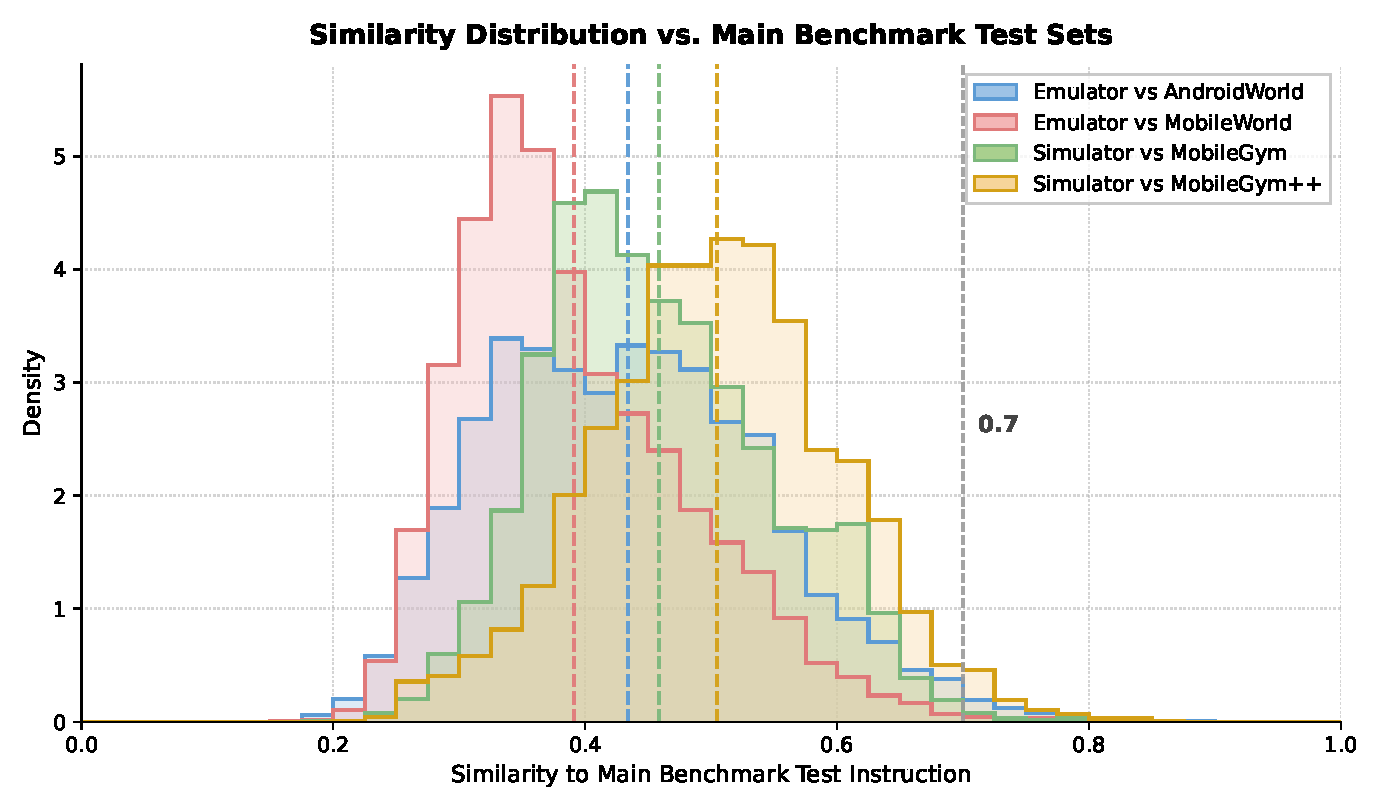
\includegraphics[width=\linewidth]{figures/openai_similarity_hist.pdf}\\[-0.2em]
{\small (a) SFT goals}
\end{minipage}\hfill
\begin{minipage}[t]{0.49\linewidth}
\centering
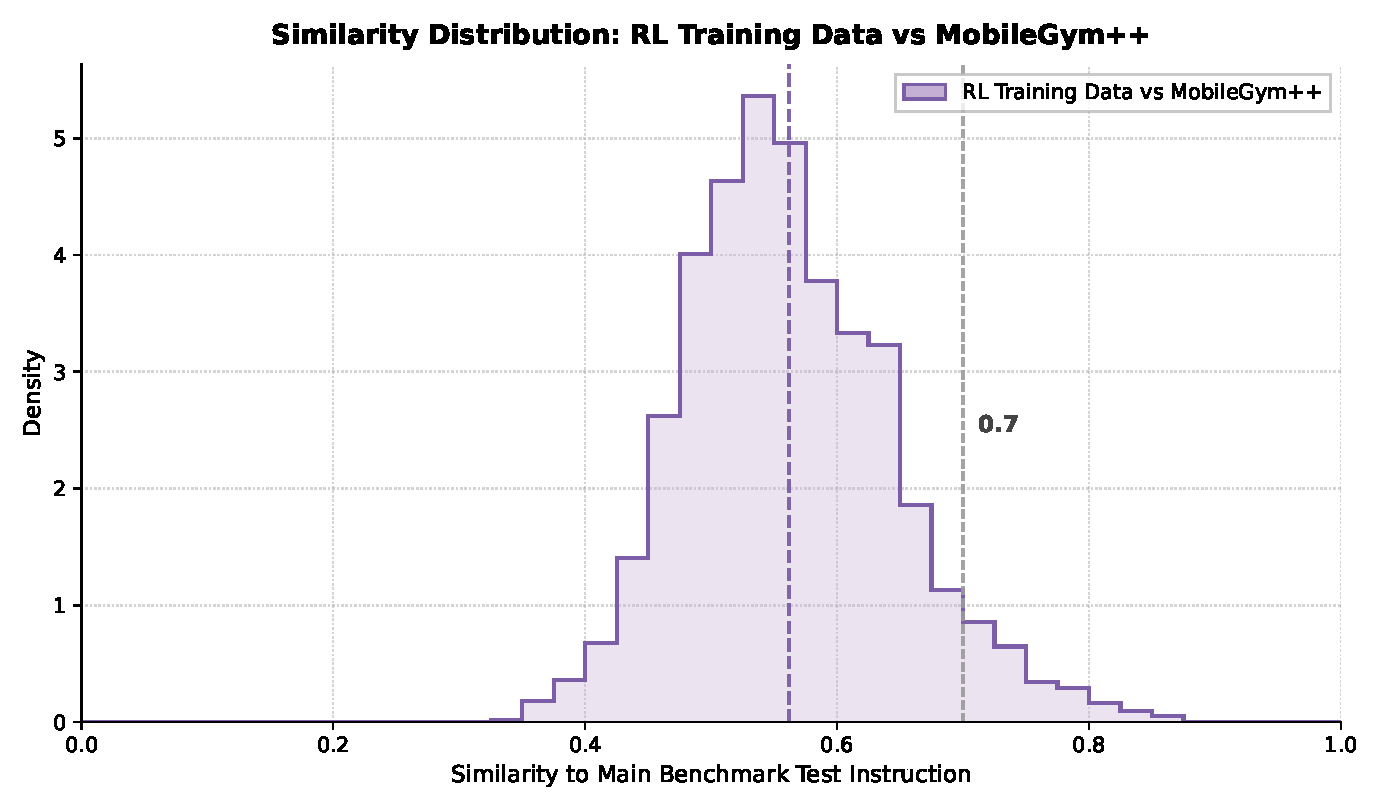
\includegraphics[width=\linewidth]{figures/openai_similarity_hist_rl_vs_mobilegympp.pdf}\\[-0.2em]
{\small (b) RL goals}
\end{minipage}
\caption{Per-goal maximum cosine similarity. (a)~SFT goals against the matched benchmark. (b)~RL task goals against \textsc{MobileGym++} Bench. Vertical lines mark each mean and the 0.7 threshold.}
\label{fig:leakage}
\end{figure}
We compare training goals with the evaluation instructions of the four benchmarks that share a runtime with training. Emulator goals (7,718 unique) are compared with AndroidWorld and MobileWorld; simulator goals (3,916 unique) are compared with MobileGym and \textsc{MobileGym++} Bench. Each goal is embedded with \texttt{text-embedding-3-large} (3,072 dimensions, L2-normalized), and we record its maximum cosine similarity to that benchmark. Table~\ref{tab:leakage} and Figure~\ref{fig:leakage}a summarize these scores. No training goal is an exact string match of an evaluation instruction, and none exceeds similarity 0.9. 

\begin{table}[h]
\centering
\small
\caption{Maximum cosine similarity of each SFT training goal to the matched benchmark. Above 0.7 counts goals whose maximum exceeds 0.7.}
\label{tab:leakage}
\begin{tabular}{lrrrr}
\toprule
Benchmark & Train goals & Mean & Max & Above 0.7 \\
\midrule
AndroidWorld & 7,718 & 0.434 & 0.892 & 1.11\% (86) \\
MobileWorld & 7,718 & 0.391 & 0.851 & 0.39\% (30) \\
MobileGym & 3,916 & 0.458 & 0.826 & 0.46\% (18) \\
\textsc{MobileGym++} Bench & 3,916 & 0.504 & 0.861 & 2.25\% (88) \\
\bottomrule
\end{tabular}
\end{table}


The same embedding is applied to the 2,475 RL task goals, compared only with \textsc{MobileGym++} Bench (Figure~\ref{fig:leakage}b). Exact string overlap is again zero, and none exceeds 0.9. The mean maximum similarity is 0.562, the maximum is 0.862, and 6.1\% (151) exceed 0.7.





\section{MobileGym++ App Construction}
\label{app:mgpp-build}

\paragraph{Behavior specification.}
We represent core application workflows as a structured graph of page nodes and meaningful UI states. Each state-changing interaction names its UI element and action, describes the expected state effect, and includes a check for the resulting state. This makes navigation and business-state writes explicit before implementation. The specification is then used as the contract for implementing and checking routes, actions, and state changes.

\par\medskip
\noindent
\begin{minipage}{\linewidth}
\centering
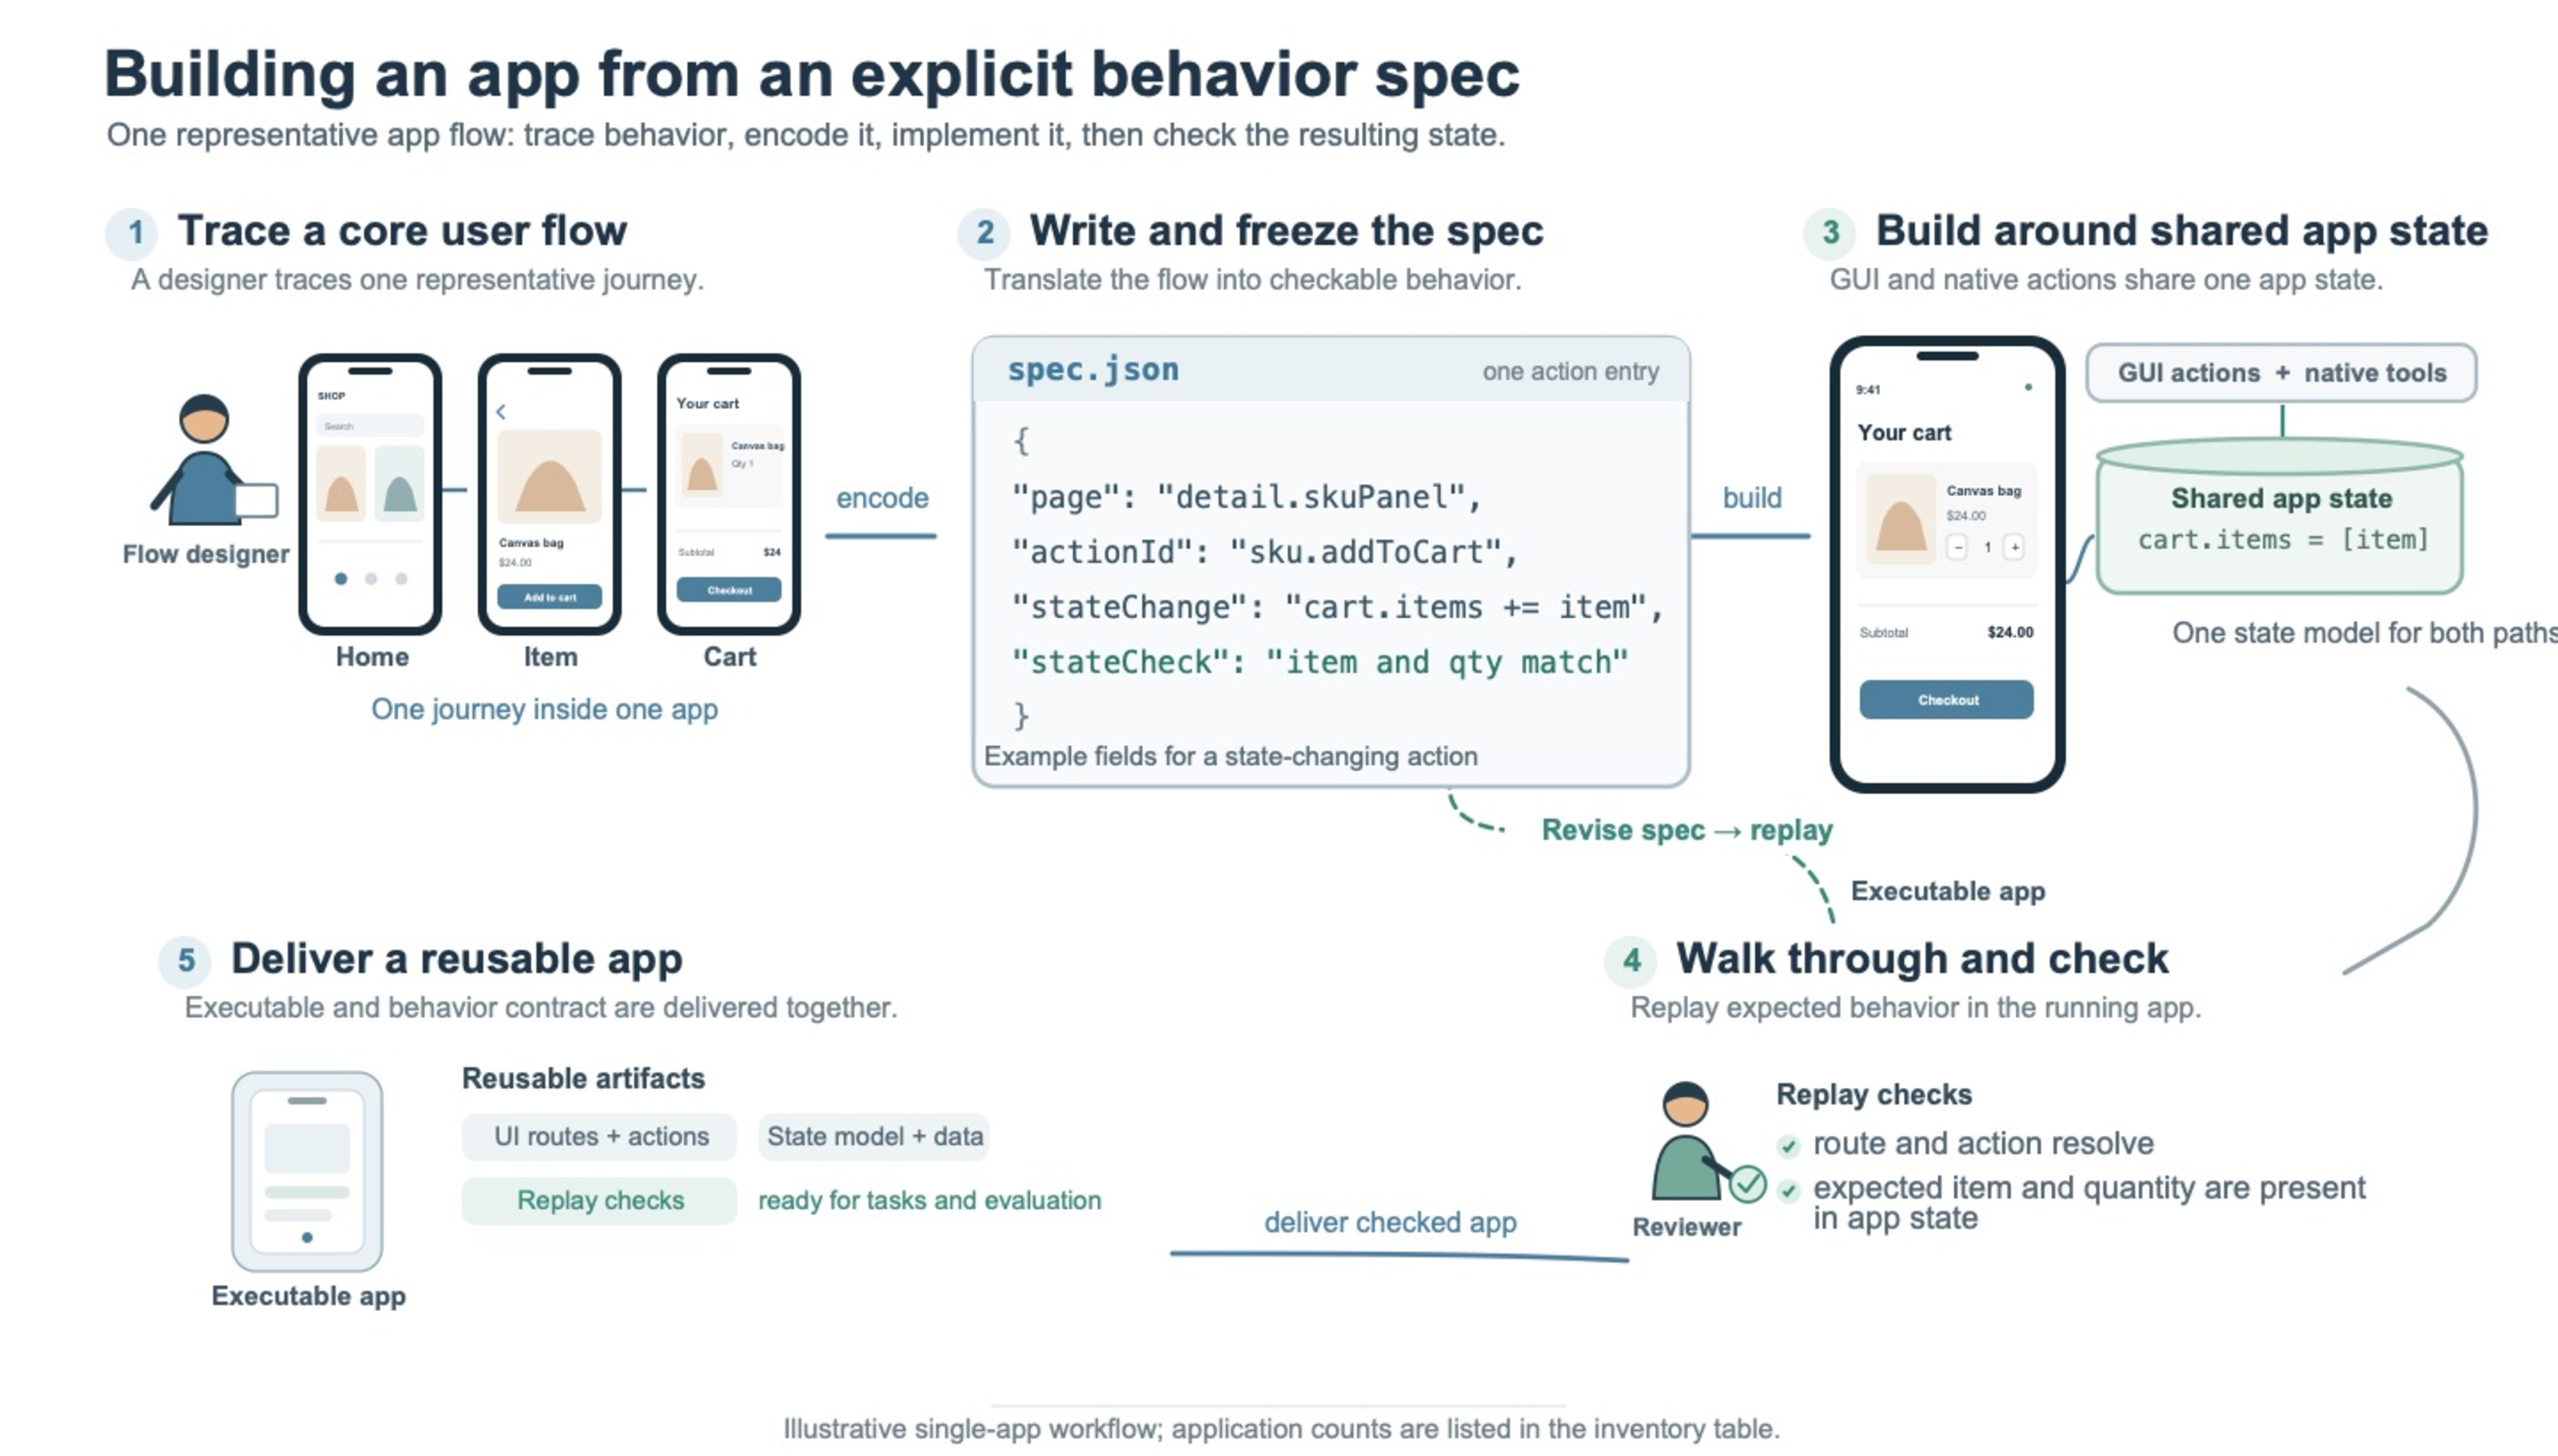
\includegraphics[width=\linewidth]{figures/app-construction-process.pdf}
\captionof{figure}{Illustrative single-app workflow. The phone screens show one journey; the numbered circles mark construction stages, not application counts.}
\label{fig:app-construction-process}
\end{minipage}
\par\medskip

\paragraph{Specification entry.}
The excerpt below shows the form of a state-changing interaction. A page identifier groups its controls; the action identifier names the operation; and the state change and check make the outcome observable.
\begin{minipage}{\linewidth}
\begin{lstlisting}[basicstyle=\ttfamily\small, frame=single, columns=fullflexible, breaklines=true]
{
  "id": "detail.skuPanel",
  "interactions": [{
    "element": "Add to cart",
    "effect": "state",
    "actionId": "sku.addToCart.confirm",
    "stateChange": "cart.items += item",
    "stateCheck": "item and quantity match"
  }]
}
\end{lstlisting}
\end{minipage}

\paragraph{Implementation and checks.}
Routes and actions operate on app-owned state and seeded data. GUI actions and app-native tools use the same app state. A coverage check maps declared interaction identifiers to implementation bindings; runtime replay checks representative transitions and their expected state effects. When a mismatch appears, the specification is corrected and the affected checks are replayed. Each delivered app includes its executable interface, state model, seeded data, and reusable checks for core flows. Benchmark instructions and terminal verifiers are authored separately on top of the completed apps.


\section{Playground Inventory}
\label{app:mgpp-apps}

\textsc{MobileGym++} contains 63 installable simulated clients: 35 applications built in this work and 28 inherited from MobileGym. Of these, 47 are commercial-style applications and 16 are system clients. The Android emulator inventory contains 62 applications. The tables below list applications by domain; the emulator inventory is not divided by source batch.

\begin{table}[H]
\centering
\small
\caption{Application counts by domain in the two runtimes.}
\label{tab:app-domain-counts}
\begin{tabular}{lrr}
\toprule
Domain & \textsc{MobileGym++} & Emulator \\
\midrule
Lifestyle & 18 & 19 \\
Productivity & 15 & 23 \\
Entertainment & 9 & 15 \\
Shopping & 8 & 1 \\
Travel & 5 & 3 \\
Social & 6 & 0 \\
Finance & 2 & 1 \\
\midrule
Total & 63 & 62 \\
\bottomrule
\end{tabular}
\end{table}

\subsection{MobileGym++ applications}
\label{app:mgpp-app-table}

Table~\ref{tab:app-mgpp-list} gives the complete 63-client inventory; $^\ast$ marks the 35 applications built in this work.

\begin{table}[H]
\centering
\small
\caption{The 63 \textsc{MobileGym++} clients. $^\ast$ marks the 35 applications built in this work and $^\dagger$ marks the 16 system clients.}
\label{tab:app-mgpp-list}
\begin{tabular}{lp{0.74\linewidth}}
\toprule
Domain & Applications \\
\midrule
Lifestyle (18) & Baicizhan$^\ast$, Cainiao$^\ast$, Dianping$^\ast$, Keep$^\ast$, Luckin Coffee$^\ast$, Maoyan$^\ast$, Meituan$^\ast$, Meiyou$^\ast$, Weather$^\dagger$, Answer Sheet$^\dagger$, Browser$^\dagger$, Calculator$^\dagger$, Calculator~2$^\dagger$, Clock$^\dagger$, Compass$^\dagger$, Gallery$^\dagger$, Settings$^\dagger$, Themes$^\dagger$ \\
Productivity (15) & BOSS Zhipin$^\ast$, Days Matter$^\ast$, TickTick$^\ast$, Fanqie ToDo$^\ast$, flomo$^\ast$, Google Drive$^\ast$, Mail$^\ast$, Slack$^\ast$, Daily$^\ast$, Tencent Meeting, Calendar$^\dagger$, Phone$^\dagger$, Files$^\dagger$, Notes$^\dagger$, Messages$^\dagger$ \\
Entertainment (9) & Podcasts$^\ast$, Fanqie Novel$^\ast$, Tencent Video$^\ast$, NetEase Cloud Music$^\dagger$, Ximalaya$^\ast$, Youku$^\ast$, Bilibili, Spotify, WeRead \\
Shopping (8) & JD$^\ast$, Pinduoduo$^\ast$, Suning$^\ast$, Taobao$^\ast$, Taobao Instant Commerce$^\ast$, Vipshop$^\ast$, Xianyu$^\ast$, eBay \\
Travel (5) & Ctrip$^\ast$, DiDi$^\ast$, Qunar$^\ast$, Maps, Railway 12306 \\
Social (6) & Douban$^\ast$, Weibo$^\ast$, RedNote, Reddit, WeChat, X \\
Finance (2) & Alipay, Kapi$^\ast$ \\
\bottomrule
\end{tabular}
\end{table}

\subsection{Emulator applications}
\label{app:emu-apps}

\begin{table}[H]
\centering
\small
\caption{The 62 Android emulator applications, grouped by domain. AndroidWorld and MiniWoB denote the task-support apps installed with the AndroidWorld suite.}
\label{tab:app-emu-list}
\begin{tabular}{lp{0.74\linewidth}}
\toprule
Domain & Applications \\
\midrule
Lifestyle (19) & Camera, Chrome, Clock, Settings, Simple Gallery Pro, AndroidWorld, Broccoli, Clipper, MiniWoB, OpenTracks, APKPure, Breezy Weather, Coursera, DuckDuckGo, F-Droid, NerdCalci, Snapseed, Quark, Xiachufang \\
Productivity (23) & Files, Contacts, Dialer, Simple SMS Messenger, Simple Calendar Pro, Joplin, Markor, Tasks, Simple Draw Pro, Audio Recorder, Amaze, Material Files, MiXplorer, MT Manager, Etar, Omni Notes FOSS, Code Editor, DeepL, GeminiAssist, Doubao, Element, Mattermost, Session \\
Entertainment (15) & VLC, Retro Music, iQIYI, Youku, Bilibili, NetEase Cloud Music, NewPipe, AntennaPod, Toutiao, Yahoo News, Yahoo Sports, Wikipedia, Librera, 2048, Angry Birds Friends \\
Shopping (1) & eBay \\
Travel (3) & OsmAnd, Booking.com, Citymapper \\
Finance (1) & Pro Expense \\
\bottomrule
\end{tabular}
\end{table}

\section{Data Collection}
\label{app:data}

\subsection{Construction details}
\label{app:sft-data}

\paragraph{Environment representation and task synthesis.}
Task synthesis is grounded in the functions an application supports and the states reachable from a given screen. For Android emulator applications, exploration is used to map screens and transitions. For \textsc{MobileGym++}, the page, action, and business-object declarations are available from each simulated client. A global view summarizes an application's features and where they are located; a local view lists states directly reachable from the current screen. Instructions are phrased as user goals rather than naming the controls, tools, or verifier fields to use.

\paragraph{Trajectory rollout and filtering.}
The same model executes each instruction step by step, producing a \texttt{Thought:} paragraph followed by one action per turn. When the foreground application exposes app-native tools, its tool catalog is available and the model may choose a tool call or GUI action. Both channels act on the same application state. A rollout is retained when the task succeeds under its runtime-specific check: the programmatic verifier for \textsc{MobileGym++} or a vision-language judge for Android emulator tasks. Degenerate transitions that leave application state unchanged are removed.

\subsection{Executable RL tasks}
\label{app:rl-data}
Each executable RL task is a triple of instruction, initial state, and verifier. The initial state is a snapshot of the \textsc{MobileGym++} application stores, so repeated rollouts of a task start from the same state. The verifier compares application state before and after an episode and checks whether the requested change was written. Since it reads application state rather than the screen, it evaluates GUI and app-native tool actions alike.

\subsection{Data composition}
\label{app:data-quality}

\paragraph{Source coverage.}
The SFT mixture contains 11,643 trajectories. Of these, 7,725 come from emulator(about two third), while 3,918 come from simulator (about one third; Table~\ref{tab:app-sft-data}). The mixture therefore combines trajectories from Android emulator applications with controllable simulated-client workflows.

\paragraph{Trajectory length and action channels.}
Mean trajectory lengths range from 6.8 steps for hybrid trajectories to 11.9 for AndroidWorld, with MobileGym at 10.7 and MobileWorld at 8.8. The 1,774 hybrid trajectories use app-native tools alongside GUI actions.

\section{MobileGym++ Bench}
\label{app:mgpp-bench}

The following subsections document the task split and domain distribution for MobileGym++ Bench, and give two worked examples that illustrate the evaluation protocol concretely.

\subsection{Task composition}
\label{app:mgpp-bench-split}
The 215 tasks span one to four applications. Of these, 109 use one app, 74 use two, 27 use three, and 5 use four; 106 tasks therefore require cross-app interaction. Figure~\ref{fig:bench-composition} and Table~\ref{tab:bench-domain-incidence} report the same split and the task incidences by domain. Because a cross-domain task is counted once in each domain it touches, these incidences overlap and do not sum to 215.

\begin{figure}[t]
\centering
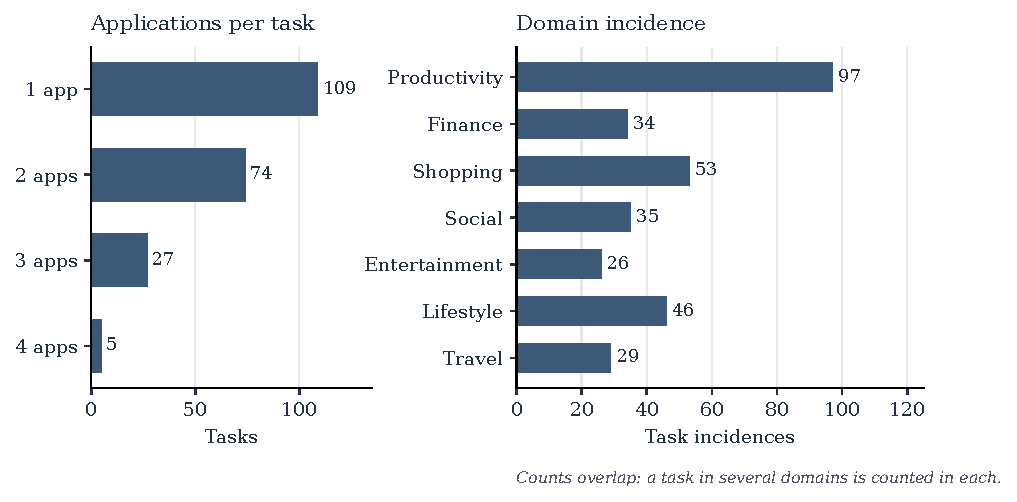
\includegraphics[width=\linewidth]{figures/fig_bench_composition.pdf}
\caption{MobileGym++ Bench composition. Left: tasks by the number of applications they touch. Right: task incidences by domain. Domain counts are not mutually exclusive.}
\label{fig:bench-composition}
\end{figure}

\begin{table}[t]
\centering
\small
\caption{MobileGym++ Bench task incidences by domain. A task that touches more than one domain is counted in each, so the column does not sum to 215.}
\label{tab:bench-domain-incidence}
\begin{tabular}{lr}
\toprule
Domain & Task incidences \\
\midrule
Productivity & 97 \\
Finance & 34 \\
Shopping & 53 \\
Social & 35 \\
Entertainment & 26 \\
Lifestyle & 46 \\
Travel & 29 \\
\bottomrule
\end{tabular}
\end{table}

\subsection{Example tasks}
\label{app:mgpp-bench-ex}

\paragraph{GUI-only: transfer search results into Notes.}
Task 202 (\texttt{HTV6Case27}) asks the agent to search RedNote (Xiaohongshu) using the Chinese term for travel, identify the two most-liked posts among the first ten results, and write their full titles to the system Notes app, one per line (not to flomo). In the GUI-only setting, the agent can use the \texttt{mobile\_use} interface actions but receives no app-native tools. The programmatic checker independently retrieves the top two titles from the initial search results and verifies that both appear in the latest Notes entry.

\paragraph{Hybrid: complete a Taobao purchase.}
Task 111 (\texttt{HTV6Case69}) asks the agent to buy a Jianmu large-capacity insulated flask made of 316 stainless steel, choose the saved address marked School, and pay using Huabei installments. The hybrid action set combines GUI actions with Taobao app-native tools; relevant calls include \texttt{taobao\_\_search\_items}, \texttt{taobao\_\_get\_item\_summary}, and \texttt{taobao\_\_add\_to\_cart}. \texttt{taobao\_\_prepare\_checkout} opens the confirmation page as a non-persisted draft, so the agent must still complete the payment flow in the GUI. The checker requires a new paid order for the target item, with the school-tagged address and Huabei installment payment recorded in the order.

\section{App-native tool examples}
\label{app:tool-schema}
App-native tools occupy the same action slot as \texttt{mobile\_use} GUI interactions: at each step, the agent chooses one action from a single list that includes both. When an application is in the foreground, its tool catalog is appended to that list; when the application leaves the foreground, its tools are removed. The following Taobao schemas illustrate read, state-changing, and navigation-to-GUI operations. The tool handlers and the visible application use the same \texttt{useTaobaoStore}: for example, \texttt{add\_to\_cart} updates the cart state that the GUI renders. Tool schemas reject undeclared input keys.

\begin{lstlisting}[basicstyle=\ttfamily\small,frame=single,breaklines=true]
taobao__search_items(query: string, limit?: integer)
taobao__get_item_summary(item_id: string)
taobao__add_to_cart(item_id: string, sku_description: string,
                    quantity: integer [1..99])
taobao__prepare_checkout(cart_line_ids: string[1..30])
\end{lstlisting}

The first two calls read the catalog; \texttt{add\_to\_cart} validates the item, SKU, and quantity before writing the shared cart. \texttt{prepare\_checkout} accepts one to 30 valid cart-line IDs, opens the confirmation page, and creates neither an order nor a payment. The GUI then continues from the same app state.

\section{System prompt}
\label{app:sys-prompt}

The prompt below is the evaluation harness for Qwen3.5-9B, Qwen3.6-27B, and the OpenMobile-2 checkpoints trained from them. It is used in both the GUI-only and hybrid settings. The GUI tool \texttt{mobile\_use} is always available; when an application exposes app-native tools, the environment lists them in the tool message for as long as that application stays in the foreground. In the GUI-only setting no such catalog is attached. Results marked $*$ for other models in Table~\ref{tab:main} are reproduced by us, but not with this harness. Each of those models keeps its own action format and system prompt.

\promptfile{System prompt for Qwen and OpenMobile-2 evaluation}{prompts/system_prompt.txt}
